\chapter{周期信号的傅里叶级数}
\label{chap:fourier-series}

\keyterm{傅里叶级数}把周期信号展开成一组彼此正交的正弦或复指数。\red{展开系数给出离散谐波线谱}，后面的傅里叶变换、LTI 系统频率响应和滤波分析都从这里出发。

\section{数学准备}
\label{sec:fourier-inner-product-foundations}

内积、正交基、投影系数和 Gram--Schmidt 正交化见第一章\cref{sec:inner-product-foundations}。这里直接把这些结果用于周期区间上的\keyterm{傅里叶基}。

\section{周期信号的三角傅里叶级数}
\label{sec:trigonometric-fourier-series}

设 $x(t)$ 以 $T_0>0$ 为周期，即 $x(t+T_0)=x(t)$，\keyterm{基本角频率}为
\begin{equation}
  \omega_0=\frac{2\pi}{T_0}.
  \label{eq:fundamental-angular-frequency}
\end{equation}
\keyterm{三角形式的傅里叶级数}写作
\begin{equation}
  x(t)=B_0+\sum_{n=1}^{\infty}
  \bigl[B_n\cos(n\omega_0t)+C_n\sin(n\omega_0t)\bigr].
  \label{eq:trigonometric-fourier-series}
\end{equation}
系数可在任意完整周期上计算；取 $[t_0,t_0+T_0]$ 时，
\begin{align}
  B_0&=\frac{1}{T_0}\int_{t_0}^{t_0+T_0}x(t)\dd t,\\
  B_n&=\frac{2}{T_0}\int_{t_0}^{t_0+T_0}x(t)\cos(n\omega_0t)\dd t,\\
  C_n&=\frac{2}{T_0}\int_{t_0}^{t_0+T_0}x(t)\sin(n\omega_0t)\dd t.
  \label{eq:trigonometric-fourier-coefficients}
\end{align}
其中 $B_0$ 是\red{一个周期内的平均值}，$B_n,C_n$ 分别记录余弦和正弦谐波的权重。取积分区间时最重要的是\blue{完整覆盖一个周期}，不一定要从 $0$ 开始。

系数中的 $1/T_0$ 与 $2/T_0$ 来自基函数的积分。以 $[0,T_0]$ 为例，
\[
  \int_0^{T_0}1\dd t=T_0,\qquad
  \int_0^{T_0}\cos^2(n\omega_0t)\dd t
  =\int_0^{T_0}\sin^2(n\omega_0t)\dd t=\frac{T_0}{2}.
\]
\red{不同谐波的乘积}以及\red{正弦、余弦之间的乘积}在完整周期上的积分为零。
将级数两边乘以 $\cos(m\omega_0t)$ 再积分，只剩
\[
  \int_0^{T_0}x(t)\cos(m\omega_0t)\dd t
  =B_m\int_0^{T_0}\cos^2(m\omega_0t)\dd t
  =\frac{T_0}{2}B_m.
\]
于是便可得到 $B_m$。同理，乘以正弦可求 $C_m$，直接积分则求 $B_0$。

\subsection{收敛条件与跳变点}

常用的 \keyterm{Dirichlet 条件}可概括为：
\begin{itemize}
  \item 在一个周期内，信号应绝对可积；
  \item 只有有限个极值；
  \item 只有有限个有限幅度的间断点。
\end{itemize}

满足这些条件时，傅里叶级数在连续点收敛到 $x(t)$，在跳变点 $t_0$ 收敛到左右极限的平均值：
\begin{equation}
  \lim_{N\to\infty}S_N(t_0)
  =\frac{x(t_0^-)+x(t_0^+)}{2}.
  \label{eq:fourier-jump-convergence}
\end{equation}
所以级数在跳变处出现 \keyterm{Gibbs 现象}并不表示计算错误；部分和会在跳变附近振荡，\red{振荡宽度随项数增加而缩小}，但\red{过冲幅度不会完全消失}。判断收敛时应区分\red{连续点取函数值，跳变点取左右平均}。

\begin{example}[对称矩形波的傅里叶级数]
  设 $x(t)$ 以 $T$ 为周期，在每个周期中心附近满足
  \[
    x(t)=
    \begin{cases}
      1, & |t|<T_1,\\
      0, & T_1<|t|<T/2,
    \end{cases}
    \qquad 0<T_1<T/2.
  \]
  该信号为偶信号，所以 $C_n=0$。取 $[-T/2,T/2]$ 为一个周期，得到
  \begin{align*}
    B_0&=\frac1T\int_{-T_1}^{T_1}1\dd t=\frac{2T_1}{T},\\
    B_n&=\frac{2}{T}\int_{-T_1}^{T_1}\cos(n\omega_0t)\dd t
    =\frac{2}{T}\left[\frac{\sin(n\omega_0t)}{n\omega_0}\right]_{-T_1}^{T_1}\\
    &=\frac{4\sin(n\omega_0T_1)}{Tn\omega_0}
     =\frac{2\sin(n\omega_0T_1)}{n\pi},\\
    C_n&=\frac2T\int_{-T_1}^{T_1}\sin(n\omega_0t)\dd t=0.
  \end{align*}
  因而
  \[
    x(t)=\frac{2T_1}{T}
    +\sum_{n=1}^{\infty}
    \frac{2\sin(2\pi nT_1/T)}{n\pi}\cos(n\omega_0t).
  \]
  例如取 $T=4T_1$，则 $\omega_0T_1=\pi/2$，
  \[
    B_0=\frac12,\quad B_1=\frac2\pi,\quad B_2=0,\quad
    B_3=-\frac{2}{3\pi},\quad B_4=0,\quad B_5=\frac{2}{5\pi}.
  \]
  于是
  \[
    x(t)=\frac12+\frac2\pi\left[
      \cos(\omega_0t)-\frac{\cos(3\omega_0t)}3
      +\frac{\cos(5\omega_0t)}5-\cdots\right].
  \]
  \Cref{fig:rectangular-fourier-series} 同时画出矩形波和有限项部分和。\hl{先用偶对称性消去正弦项}，\hl{再检查哪些余弦系数为零}。

  \begin{figure}[htbp]
    \centering
    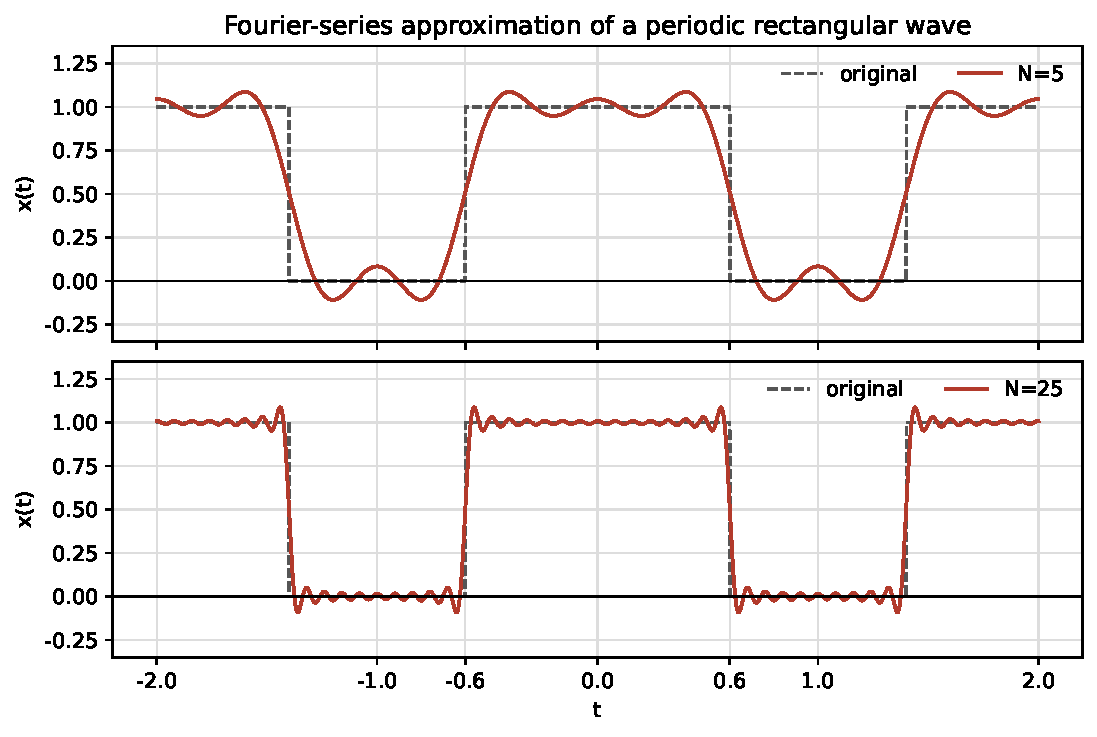
\includegraphics[width=0.86\textwidth]{05-fourier-series/rectangular-fourier-series.pdf}
    \caption{对称矩形波及其傅里叶级数有限项逼近；跳变点附近出现 Gibbs 振荡。}
    \label{fig:rectangular-fourier-series}
  \end{figure}
\end{example}

\section{复指数形式与系数转换}
\label{sec:complex-fourier-series}

利用欧拉公式，三角级数也可写成\keyterm{复指数形式}：
\begin{equation}
  \boxed{
    x(t)=\sum_{k=-\infty}^{\infty}A_k\e^{\iu k\omega_0t}
  },
  \qquad
  A_k=\frac{1}{T_0}\int_{t_0}^{t_0+T_0}
  x(t)\e^{-\iu k\omega_0t}\dd t.
  \label{eq:complex-fourier-series}
\end{equation}
复指数形式把\red{正、负频率统一在一个整数下标中}，通常更适合推导和变换。其系数本身是复数，\red{模表示该谐波的强度}，\red{辐角则包含相位信息}。

\blue{对实信号}，$A_{-k}=\overline{A_k}$。三角系数与复系数的关系为
\begin{align}
  B_0&=A_0,\\
  B_k&=A_k+A_{-k},\\
  C_k&=\iu(A_k-A_{-k}),\qquad k>0,
  \label{eq:fourier-coefficient-conversion-forward}
\end{align}
反过来，
\begin{equation}
  A_k=\frac{B_k-\iu C_k}{2},
  \qquad
  A_{-k}=\frac{B_k+\iu C_k}{2},
  \qquad k>0.
  \label{eq:fourier-coefficient-conversion-inverse}
\end{equation}
若信号是偶函数，则 $C_k=0$；若信号是奇函数，则 $B_0=B_k=0$。这些对称性\hl{在积分前直接消去一半系数}。

对前面的矩形波，复指数系数也可直接积分。$k\ne0$ 时，
\begin{align*}
  A_k&=\frac1T\int_{-T_1}^{T_1}\e^{-\iu k\omega_0t}\dd t
      =\frac1T\left[\frac{\e^{-\iu k\omega_0t}}{-\iu k\omega_0}\right]_{-T_1}^{T_1}\\
     &=\frac{\e^{\iu k\omega_0T_1}-\e^{-\iu k\omega_0T_1}}
             {\iu k\omega_0T}
      =\frac{\sin(k\omega_0T_1)}{k\pi}.
\end{align*}
$k=0$ \hl{须单独积分}，$A_0=2T_1/T$。该信号满足 $A_{-k}=A_k$，\hl{把正负频率配对}可得
\[
  A_k\e^{\iu k\omega_0t}+A_{-k}\e^{-\iu k\omega_0t}
  =2A_k\cos(k\omega_0t),
\]
与三角形式的 $B_k=2A_k$ 一致。

\begingroup
\raggedbottom

\section{傅里叶级数的性质}
\label{sec:fourier-series-properties}

已知一个周期信号的系数后，平移、反转或叠加信号时，可以直接求新系数。以下沿用\cref{eq:complex-fourier-series} 的约定，记
\[
  x(t)=\sum_{k=-\infty}^{\infty}A_k\e^{\iu k\omega_0t},
  \qquad
  y(t)=\sum_{k=-\infty}^{\infty}D_k\e^{\iu k\omega_0t},
  \qquad \omega_0=\frac{2\pi}{T_0}.
\]
两个信号参与同一运算时，须\blue{选用共同的参考周期} $T_0$；它可以大于各自的基本周期。若两个基本周期之比为无理数，其和或乘积一般不再是周期信号，不能直接使用同一组谐波下标。

\subsection{线性、平移与对称性}
\label{subsec:fs-basic-properties}

\cref{tab:ctfs-properties} 汇集常用的系数变换。表中 $\alpha,\beta$ 为常数，$m$ 为整数。
\begin{table}[H]
  \centering
  \caption{连续时间傅里叶级数的常用性质}
  \label{tab:ctfs-properties}
  \begingroup
  \renewcommand{\arraystretch}{1.5}
  \begin{tabular}{c c c}
    \toprule
    性质 & 时域信号 & 级数系数 \\
    \midrule
    线性 & $\alpha x(t)+\beta y(t)$ & $\alpha A_k+\beta D_k$ \\
    时间平移 & $x(t-t_0)$ & $A_k\e^{-\iu k\omega_0t_0}$ \\
    谐波调制 & $\e^{\iu m\omega_0t}x(t)$ & $A_{k-m}$ \\
    时间反转 & $x(-t)$ & $A_{-k}$ \\
    共轭 & $x^*(t)$ & $A_{-k}^*$ \\
    时间伸缩 & $x(\lambda t),\ \lambda>0$ & $A_k$，基频改为 $\lambda\omega_0$ \\
    时间微分 & $x'(t)$ & $\iu k\omega_0A_k$ \\
    \bottomrule
  \end{tabular}
  \endgroup
\end{table}

例如时间平移时，直接在展开式中代入 $t-t_0$：
\[
  x(t-t_0)=\sum_k
  \left(A_k\e^{-\iu k\omega_0t_0}\right)\e^{\iu k\omega_0t}.
\]
每个谐波的系数都多了一个相位因子，模保持不变，所以\red{时移只改变各谐波的相位}。谐波调制则把频率 $k\omega_0$ 移到 $(k+m)\omega_0$，相应系数下标平移。

时间伸缩须连同基频一起解释：
\[
  x(\lambda t)=\sum_k A_k\e^{\iu k(\lambda\omega_0)t}.
\]
以新周期 $T_0/\lambda$ 展开时，\red{系数不变，谐波间隔改变}，不额外乘 $1/\lambda$。若 $\lambda<0$，先按 $|\lambda|$ 伸缩，再用时间反转得到系数 $A_{-k}$。

共轭与反转性质还给出：实信号满足 $A_{-k}=A_k^*$；\red{实偶信号的系数实且偶，实奇信号的系数纯虚且奇}。

表中的微分公式对连续、分段光滑的周期信号可由分部积分得到；若信号有跳变，则导数须包含跳变处的冲激，按广义函数解释，不能只对各段求导。

\subsection{相乘与周期卷积}
\label{subsec:fs-product-periodic-convolution}

两个同周期信号相乘时，记 $x$ 中频率为 $\ell\omega_0$ 的复指数系数为 $A_\ell$，$y$ 中频率为 $(k-\ell)\omega_0$ 的复指数系数为 $D_{k-\ell}$，乘积中频率为 $k\omega_0$ 的系数为 $C_k$，则
\begin{equation}
  x(t)y(t)\quad\longleftrightarrow\quad
  C_k=\sum_{\ell=-\infty}^{\infty}A_\ell D_{k-\ell}.
  \label{eq:ctfs-product}
\end{equation}
这是\red{系数序列的普通离散卷积}。对有限级数，乘积中频率为 $k\omega_0$ 的项来自所有下标满足 $\ell+r=k$ 的组合，逐项收集就得到上式。一个周期内平方可积时，该关系可由有限部分和取均方极限得到；对每个固定 $k$，右侧求和由 Cauchy--Schwarz 不等式保证绝对收敛。

两个周期信号在全时间轴上的普通卷积通常不收敛。把积分范围限制为一个周期，定义连续时间的\keyterm{周期卷积（periodic convolution）}：
\begin{equation}
  z(t)=\int_{t_0}^{t_0+T_0}x(\tau)y(t-\tau)\dd\tau.
  \label{eq:ctfs-periodic-convolution}
\end{equation}
被积函数关于 $\tau$ 以 $T_0$ 为周期，所以积分起点可以任取。将两信号展开后，一个周期上的正交积分只保留相同谐波：
\[
  \int_{t_0}^{t_0+T_0}
  \e^{\iu(\ell-r)\omega_0\tau}\dd\tau
  =\begin{cases}
    T_0,&\ell=r,\\
    0,&\ell\ne r.
  \end{cases}
\]
于是
\begin{equation}
  z(t)=\sum_k T_0A_kD_k\e^{\iu k\omega_0t}.
  \label{eq:ctfs-periodic-convolution-coefficients}
\end{equation}
即\red{周期卷积对应系数逐项相乘}，并带有周期因子 $T_0$。本章的定义没有在积分前除以周期；若改用归一化周期卷积 $T_0^{-1}\int_{T_0}xy$，系数才是 $A_kD_k$。例如 $x=y=1$ 时，积分结果为 $T_0$，可用来核对这个因子。

\subsection{积分与直流分量}
\label{subsec:fs-integration}

设 $q'(t)=x(t)$，积分取有限起点
\[
  q(t)=q(t_0)+\int_{t_0}^{t}x(\tau)\dd\tau.
\]
每经过一个周期，
\[
  q(t+T_0)-q(t)=\int_t^{t+T_0}x(\tau)\dd\tau=T_0A_0.
\]
所以 $q$ 为周期信号的条件是\blue{输入的平均值为零}，即 $A_0=0$；非零直流分量会积累成斜坡，使积分结果失去周期性。满足零均值条件时，若 $q$ 的系数为 $Q_k$，由微分性质可得
\begin{equation}
  Q_k=\frac{A_k}{\iu k\omega_0}\quad(k\ne0),
  \qquad Q_0\text{ 由积分常数确定}.
  \label{eq:ctfs-integration}
\end{equation}
\red{零频系数须单独确定}。例如 $x(t)=\cos\omega_0t$ 的周期原函数为 $q(t)=\sin(\omega_0t)/\omega_0+C$，常数 $C$ 不由 $x$ 决定。即使均值为零，从 $-\infty$ 起算的普通反常积分仍可能不收敛，不能用它代替这里的有限起点积分。

\subsection{Parseval 关系与平均功率}
\label{subsec:ctfs-parseval}

若\blue{一个周期内平方可积}，则\keyterm{帕塞瓦尔关系（Parseval's relation）}为
\begin{equation}
  P_x=\frac1{T_0}\int_{t_0}^{t_0+T_0}|x(t)|^2\dd t
  =\sum_{k=-\infty}^{\infty}|A_k|^2.
  \label{eq:ctfs-parseval}
\end{equation}
对有限部分和，模平方展开后的交叉项在一个周期上积分为零，留下 $T_0\sum_k|A_k|^2$；再取均方极限即得上式。单个谐波 $A_k\e^{\iu k\omega_0t}$ 的平均功率为 $|A_k|^2$，因此\red{总功率等于各谐波功率之和}。对实信号，利用正负频率成对出现，还可写成
\[
  P_x=|A_0|^2+2\sum_{k=1}^{\infty}|A_k|^2
     =B_0^2+\frac12\sum_{k=1}^{\infty}(B_k^2+C_k^2).
\]
这里计算的是平均功率；非零周期信号在整个实轴上的总能量一般为无穷大，不能套用有限能量信号的频谱平方积分。

\begin{example}[平移矩形波并去掉直流分量]
  取前面占空比为 $1/2$ 的对称矩形波，以 $T_0$ 为周期，其系数为
  \[
    A_0=\frac12,\qquad A_k=\frac{\sin(k\pi/2)}{k\pi}\quad(k\ne0).
  \]
  令 $g(t)=x(t-T_0/4)-1/2$。先平移，系数乘 $\e^{-\iu k\pi/2}$；再减去常数，只改变零频项：
  \[
    G_0=0,\qquad
    G_k=\e^{-\iu k\pi/2}\frac{\sin(k\pi/2)}{k\pi}\quad(k\ne0).
  \]
  例如 $G_1=-\iu/\pi$、$G_{-1}=\iu/\pi$，偶数下标系数均为零，无须重新做分段积分。$g(t)$ 除跳变点外取 $\pm1/2$，故平均功率为 $1/4$；系数也给出
  \[
    \sum_k|G_k|^2
    =\frac{2}{\pi^2}\sum_{r=0}^{\infty}\frac1{(2r+1)^2}
    =\frac14.
  \]
  计算时可\hl{先处理平移，再调整直流项}，并用平均功率核对系数的归一化。
\end{example}

\begin{remark}[与傅里叶变换性质的对应]
  在\cref{sec:ctft-periodic-transform} 中，周期信号的变换写成
  \[
    X(\iu\omega)=2\pi\sum_k A_k\impulse(\omega-k\omega_0).
  \]
  变换的时移、反转和共轭性质作用到各条谱线上，就给出本节的系数关系。使用时仍须区分平均功率与总能量、周期卷积与普通卷积；含冲激的频谱不能直接作模平方后套入有限能量公式。
\end{remark}

\endgroup

\section{正交基、傅里叶基与其他展开}
\label{sec:fourier-orthogonal-bases}

在周期区间 $[t_0,t_0+T_0]$ 上取内积
\[
  \langle f,g\rangle
  =\int_{t_0}^{t_0+T_0}f(t)\overline{g(t)}\dd t.
\]
\keyterm{复指数族} $e_k(t)=\e^{\iu k\omega_0t}$ 满足
\begin{equation}
  \langle e_k,e_\ell\rangle
  =T_0\,\mathbf{1}_{k=\ell},
  \label{eq:fourier-exponential-orthogonality}
\end{equation}
其中 $\mathbf{1}_{k=\ell}$ 在 $k=\ell$ 时为 $1$，否则为 $0$。当 $k=\ell$，被积函数为 $1$，积分等于 $T_0$；当 $k\ne\ell$，
\begin{align*}
  \langle e_k,e_\ell\rangle
  &=\int_{t_0}^{t_0+T_0}\e^{\iu(k-\ell)\omega_0t}\dd t\\
  &=\frac{\e^{\iu(k-\ell)\omega_0t_0}}
          {\iu(k-\ell)\omega_0}
    \left[\e^{\iu(k-\ell)\omega_0T_0}-1\right]=0,
\end{align*}
因为方括号内为 $\e^{\iu2\pi(k-\ell)}-1=0$。

将 $x(t)=\sum_kA_ke_k(t)$ 与 $e_r$ 取内积，逐项计算为
\[
  \langle x,e_r\rangle=\sum_k A_k\langle e_k,e_r\rangle=T_0A_r,
  \qquad
  A_r=\frac{\langle x,e_r\rangle}{T_0},
\]
这就得到\cref{eq:complex-fourier-series}中的系数公式。傅里叶级数的系数计算可以统一理解为\red{在正交基上做投影}。

\subsection{其他常见正交基}

傅里叶基\blue{适合周期且具有全局振荡结构的信号}。在此补充其他几类的正交展开：

\begin{itemize}
  \item \keyterm{Haar 基}由局部矩形函数组成，\blue{适合表示局部突变和分段结构}；
  \item \keyterm{Legendre 多项式}在 $[-1,1]$ 上正交，定义为
  \begin{equation}
    P_n(x)=\frac{1}{2^n n!}\frac{\dd^n}{\dd x^n}(x^2-1)^n,
    \label{eq:legendre-polynomial}
  \end{equation}
  并满足
  \begin{equation}
    \int_{-1}^{1}P_m(x)P_n(x)\dd x
    =\frac{2}{2n+1}\mathbf{1}_{m=n}.
    \label{eq:legendre-orthogonality}
  \end{equation}
  因此 $f(x)=\sum_{n\geq0}a_nP_n(x)$ 时，$a_n=(2n+1)\langle f,P_n\rangle/2$；
  \item \keyterm{主成分分析（principal component analysis，PCA）}也可看作在数据向量空间中寻找一组正交方向。先去除均值 $A_0=N^{-1}\sum_{i=1}^{N}x_i$，再用正交方向 $A_1,A_2,\ldots$ 展开样本；每个系数仍由内积投影得到。与傅里叶展开的差别在于：傅里叶基由周期结构预先给定，\red{PCA 的方向则由数据本身决定}。
\end{itemize}

这些方法都先选择正交方向，再计算投影系数并重构信号。下一章把离散的谐波索引\red{推广为连续频率变量}。
